% Тема. Командная строка. 
% Показать примеры использования. Рассказать о преимуществах и недостатках в
% сравненни с графическим "оконным" интерфейсом. 
% Ознакомить с назначениме  эмулятора терминала и об реализациях.

\begin{frame}{Примеры использования командной строки}
	\begin{columns}
	\column{0.5\textwidth}
        \begin{itemize}
            \item чаты
            \item компьютерные игры Quake, DotA
            \item операционные системы
        \end{itemize}
	\column{0.5\textwidth}
	% insert picture of Quake 
    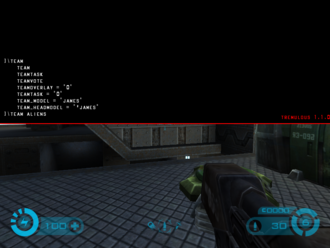
\includegraphics[height=0.4\textheight]{../../slides/cmdline/330px-Tremulous_console.png}
	\end{columns}
\end{frame}

\begin{frame}{Преимущества командной строки}
	\begin{itemize}
		\item Работа через сеть либо RS232
		\item Быстрый доступ к командам системы
		\item Легче отладка сообществом
		\item Легкость автоматизации
	\end{itemize}
\end{frame}

\begin{frame}{Недостатки командной строки}
	\begin{itemize}
		\item Oтсутствуют возможности обнаружения (discoverabililty)
		\item Необходимость изучения синтаксиса команд и запоминания сокращений.  (синтаксис может различаться)
		\item Без автодополнения, ввод длинных и содержащих спецсимволы параметров с клавиатуры может быть затруднительным
		\item Отсутствие «аналогового» ввода.
	\end{itemize}
\end{frame}

\begin{frame}{Эмуляторы терминала в графическом режиме}
	\begin{itemize}
		\item xterm
		\item rxvt
        \item gnome-terminal
        \item konsole
        \item Yakuake (Yet Another Kuake)
	\end{itemize}
\end{frame}
\note { 
Примеры приложений которые лучше выглядят в графическом режиме браузер,
редакторы видео и графики. Поэтому пользователь при работе, как правило,
совмещает оба интерфейса: использует графическое окружениe в сочетании с
интерфейсом командной строки. 
В графическом окружении интерфейса командной строки предоставляют приложения -
эмуляторы терминала. 
реализации - для графической системы X Window xterm, rxvt. Для GNOME
gnome-terminal, для KDE konsole, Yakuake (Yet Another Kuake выезжает по нажатии
тильды ~ как Quake)  
Дополнительные замечания:
Терминал - устройство для ввода вывода информации, уже устарел.
Графические приложения можно запускать из командной строки. 
}
